\documentclass[a4paper,12pt]{article}
%%%%%~~~~~~~~~~~~~~~~~~~~~usepackage~~~~~~~~~~~~~~~~~
\usepackage{rotating}
\usepackage[top=1in, bottom=1in, left=1in, right=1in]{geometry}
\usepackage{graphicx}
\usepackage[numbers,square,sort&compress]{natbib}
\usepackage{setspace}
\usepackage[cdot,mediumqspace,]{SIunits}
\usepackage{caption}
\usepackage{subcaption}
\usepackage{mathtools}
\usepackage{authblk} % to get affil
\usepackage{float} % to get figures where wanted
\usepackage{indentfirst} % to indent the first para of every chapter


%####################### new command

\newcommand{\myemail}{ayushi.singh@mail.utoronto.ca}
\newcommand{\anita}{anita.bahmanyar@mail.utoronto.ca}
\newcommand{\carly}{c.berard@mail.utoronot.ca}

%####################### Title and etc

\begin{document}
\onehalfspacing
\title{Astronomical Spectroscopy}
\author{Ayushi Singh, Anita Bahmanyar, Carly Berard}
\affil{\small {\myemail}}%, {\anita}, {\carly}}
\affil{\small Astronomy and Physics, University of Toronto, ON}
\date{4 November, 2013}
\maketitle
%\altaffiltext{1}{{\myemail}}
%\altaffilmark{1}
%####################### Abstract

\begin{abstract}
\label{abstract}
This experiment examine the spectra of various light source at different integrating time collected. Python programming language was used to manipulate the data and extract various plots. From USB2000 CCD, data was collected from Neon, Flourescent Light, Table Lamp and Sun and from 16" telescope, it was from Vega, Albiero, Enif. Neon was used to obtain pixel to wavelength solution. And halogen for telescope was used to get correct for flatfield, which does not provide good correction for stars in UV, such as Vega. In Vega, various absorbtion lines were detected, including Hydrogen Balmer series. Fe, Mg, Na and Ca were observed in Sun. Flourecent light showed presnce of Mg. 

\end{abstract}

%####################### Introduction
\section{Introduction}
\label{sec:introduction}
The purpose of this report is to learn the use of spectrograph,  understand the data extraction process of multiple spectra and to obtain results that are camparable to theoretical prediction. The raw data is introduced to various errors that changes the outcomes. This includes, dark noise, read noise, gain, random error, and flatfield.  This experiment goes though the steps required to minimize these errors and to more accurate results. 

%####################### Equipment
\section{Equipment}
\label{sec:equipment}
Two methods of data collection was used for this experiment: Ocean Optics USB2000 spectrometer provided in the lab and SBIG Self Guiding Spectrograph build in 16" telescope on the $16^{th}$ floor of McLennan Physics Building. USB2000 is a diffraction gratting based optical instrument. It recieves photon from a source through a fiber and converts the power from analog to digital unit. Therefore, outputting an one-dimensional CCD detector array \cite{instructions}. This array is observed using the SpectraSuite software installed in lab computers. This software gives the user freedom to change exposure time before each reading. The other instrument is 16", reflector, computer-operated telescope. It has build in spectroscope that was used to collect data though vaious software, incuding TheSky and Maestro to operate the telescope and Maxium-DL to control the CCD camera \cite{telescope}. Here also, user had ability to change the exposure time.

%####################### Data
\section{Data Summary}
\label{sec:data}
Data was collected from USB2000 was from Neon light, Table lamp, Fluorescent Bulb and the Sun, with different sample size and expourse time. All three group memebers contributed equally in this data collection process. However, there were few issues. The lab room is bright even with blinds down and therefore it introduces extra photon in the detector. One of the solution was to place the optical fiber and the light source in a cupboard. Another issue was that the data was obtained with one person holding the fiber in front of source. This gave us many human error, which was explictly presented in our data. The way around it was to stick the fiber to the source using tape and avoid all contact while taking data.  However, both of these solutions can not be used for the Bulb and the Sun. Following is the table with data summary. 
%~~~~~~~~~~~~~~~~~~~~~~~~~~~~~~~~~~~~ CCD ~~~~~~~~~~~~~~~~~~~~~~~~~~~~~~~~~~~~~~~~~~~~
\begin{table}[H]
\centering % used for centering table
\caption{Data from the CCD in the lab}
\tabcolsep 2.pt %\small
\footnotesize

\begin{tabular}{ccccc}% centred columns (8 columns)
\hline
\hline

Data Number  & Source & Exposure Time & Number of Samples & Comments \\
& & (ms) & &\\

 
\hline
\hline

1   &   Lamp            & 50     & 10   &\\
2   &   Lamp            & 100    & 1000 & to calculate gain and noise\\
3   &   Lamp            & 200    & 10   &\\
4   &   Lamp            & 1000   & 10   &\\
5   &   Neon            & 100    & 1000 & pixel to wavelength relation\\
6   &   Fluorescent Light& 100    & 6    & mercury light\\
7   &   Sun             & 100    & 6    &\\
8   &   Dark            & 50     & 10   &\\
9   &   Dark            & 100    & 10   &\\
10  &   Dark            & 200    & 10   &\\
11  &   Dark            & 1000   & 10   &\\

\hline
\hline

\end{tabular}
\label{table:ccd} % is used to refer this table in the text
\end{table}
%~~~~~~~~~~~~~~~~~~~~~~~~~~~~~~~~~~~~~~~~~~~~~~~~~~~~~~~~~~~~~~~~~~~~~~~~~~~~~~~~~~~~~~~~~~
Data collection from telescope was a group effort. Over two nights different sets of data was collected. In this report, only the data from the first night will be used. With the help of Michael Williams, Observatory Demonstrator at University of Toronto, data was collected from Vega, Erif and Albireo as a group, where as Halogen and Neon was provided by Michael Williams. For all the data took from telescope, corresponding dark count data is was also collected. This was then used to reduce noise from the Data. Biggest issue was light polution from the city light. Following is the data summary.
%~~~~~~~~~~~~~~~~~~~~~~~~~~~~~~~~~~~~ Telescope ~~~~~~~~~~~~~~~~~~~~~~~~~~~~~~~~~~~~~~~~~~~~ figure
\begin{table}[H]
\centering % used for centering table
\caption{Data from the campus Telescope}
\tabcolsep 2.pt %\small
\footnotesize

\begin{tabular}{cccc}% centred columns (8 columns)
\hline
\hline

Data Number & Source & Exposure Time & Comments \\
& & (s) &\\

 
\hline
\hline
1   &   Vega    &  15  & \\
2   &   Vega    &  30  & \\
3   &   Vega    &  60  & \\
4   &   Enif    &  30  &\\
5   &   Enif    &  60  &\\
6   &   Albireo01&  60  & one star from the binary system\\   
7   &   Albireo02&  60  & second star from the binary system\\
8   &   Halogen &  300    & used to correct for flatfield \\
9   &   Neon    &  120    & give us pixel to wavelength relationship\\


\hline
\hline

\end{tabular}
\label{table:telescope} % is used to refer this table in the text
\end{table}
%~~~~~~~~~~~~~~~~~~~~~~~~~~~~~~~~~~~~~~~~~~~~~~~~~~~~~~~~~~~~~~~~~~~~~~~~~~~~~~~~~~~~~~~~~~

%####################### Data Reduction and Method
\section{Data Reduction and Method}
\label{sec:reduction}
All the data collected from both the instuments had corresponding dark counts with them as mentioned in Section \ref{sec:data}. Dark count were collected when detecter is not pointing to any light source. This gives us information about hot pixels and error caused due to heating up of the detector. To reduce the error, these dark counts were substrated from the raw data. Then, data was converted from pixel to wavelength using python module: \textit{scipt.optimize.leastsq} \cite{scipy}. This outputs wavelength solution with minimized residuals. Two types of files .txt and .csv are easily open using \textit{numpy} python module. However, .fit files were views using DS9 software, and the data was excrated from them using \textit{pyfit} python module. 

%########## Lab CCD based calcuation
\subsection{Noise and Gain in CCD data} 
\label{sec:noise_ccd}
In USB2000, multiple sets of data was collected for each type of source, see table \ref{table:ccd}. To obtain a better result all the spectra from same source and with same exposure time were averaged using the equation,  
%~~~~~~~~~~~~~~~~~~~~~~~~~~~~~~~~~~~~
\begin{equation}
\label{eq:mean}
\bar{x} = \frac{\sum x_i}{N},
\end{equation}
where $\bar{x}$ is the mean and $N$ is number of samples. This is the average value of each pixel $x$ \cite{error}. For certiain data, variance was also calculated using, 
%~~~~~~~~~~~~~~~~~~~~~~~~~~~~~~~~~~~~
\begin{equation}
\label{eq:variance}
s^2_{ADU} = \frac{\sum x_i - \bar{x}}{N-1},
\end{equation}
where $s^2_{ADU}$ is the variance. This value represents the standard deviation (uncertainty in the measurement) squared for that data set \cite{error}. Relation between variance and mean are repesented by the equation, 
%~~~~~~~~~~~~~~~~~~~~~~~~~~~~~~~~~~~~
\begin{equation}
\label{eq:gain}
s^2_{ADU} = s^2_0 + k\bar{x}_{ADU},
\end{equation}
$s^2_0$ values give us the read noice and $k$ is $\frac{1}{gain}$ \cite{instructions}. Read noise is a constant additive measurement that needs to be subtracted from all the data before further calculations. Gain, on the other hand, gives the conversion from photoelectron to analog to digital unit (ADU). This value is 1 when one photon give one electon. 
%~~~~~~~~~~~~~~~~~~~~~~~~~~~~~~~~~~~~

%##########Telescope based calcuation 
\subsection{Calibration in Telescope Data} 
\label{sec:noise_tele}
All the data collected from the telescope have only one data for each source; therefore, mean is not used. However each data was calibrated using halogen lamp. This gave $P_i$, the calibrated intensity for each pixel using following equation \cite{instructions}, 
%~~~~~~~~~~~~~~~~~~~~~~~~~~~~~~~~~~~~
\begin{equation}
\label{eq:blackbody}
P_i = {\frac{R_i-D_{Ri}}{L_i-D_{Li}}B(\nu_i,T)},
\end{equation}
where $R_i$ is the raw signal, $L_i$ is the Lamp, $D_{Ri}$ and $D_{Li}$ is the dark count for raw signal and halogen lamp, respectivaly from Table \ref{table:telescope}. $B_{\nu}(T)$ is the Planck fucntion expresses as,   
%~~~~~~~~~~~~~~~~~~~~~~~~~~~~~~~~~~~~
\begin{equation}
\label{eq:planck}
B(\nu,T) = {\frac{2h\nu^3}{c^2}\frac{1}{exp(h\nu/kT)-1}},
\end{equation}
where $\nu_i=c/\lambda_i$, $\lambda_i$ being the corresponding wavelength for each pixel. The value for $T$ for halogen lamp is approxmitaly 3200 K. This took care of the flatfield and gives data with new intensity. This gave proper blackbody for each star that can be used to estimate the approximate surface temperature (T) of the star using the Wein's Law.
%~~~~~~~~~~~~~~~~~~~~~~~~~~~~~~~~~~~~
\begin{equation}
\label{eq:wein}
\lambda_{max} T = 0.00298,
\end{equation}
where $\lambda_{max}$ is the wavelength where peak of the star blackbody occurs. 

%####################### Calculation and Modeling
\section{Calculation and Modeling}
\label{sec:calc}

%##########Pixel to Wavelength Relation
\subsection{Pixel to Wavelength Relation} 
\label{sec:p-w}
All the data collected was in given in terms of pixels. It was changed in the proper wavelenth by using Neon data from CCD and telescope. 1000 sample od Neon was averaged using equation \ref{eq:mean} and plotted that exhibited various profound emission lines. Using python, these peaks were recoded and compared with the theoretical results \cite{Neon}.

%~~~~~~~~~~~~~~~~~~~~~~~~~~~~~~~ Figure ~~~~~~~~~~~~~~~~~~~~~~~~~~~~~~~~~~~~~~~~~~~~~~~
\begin{figure}[H]
\centering
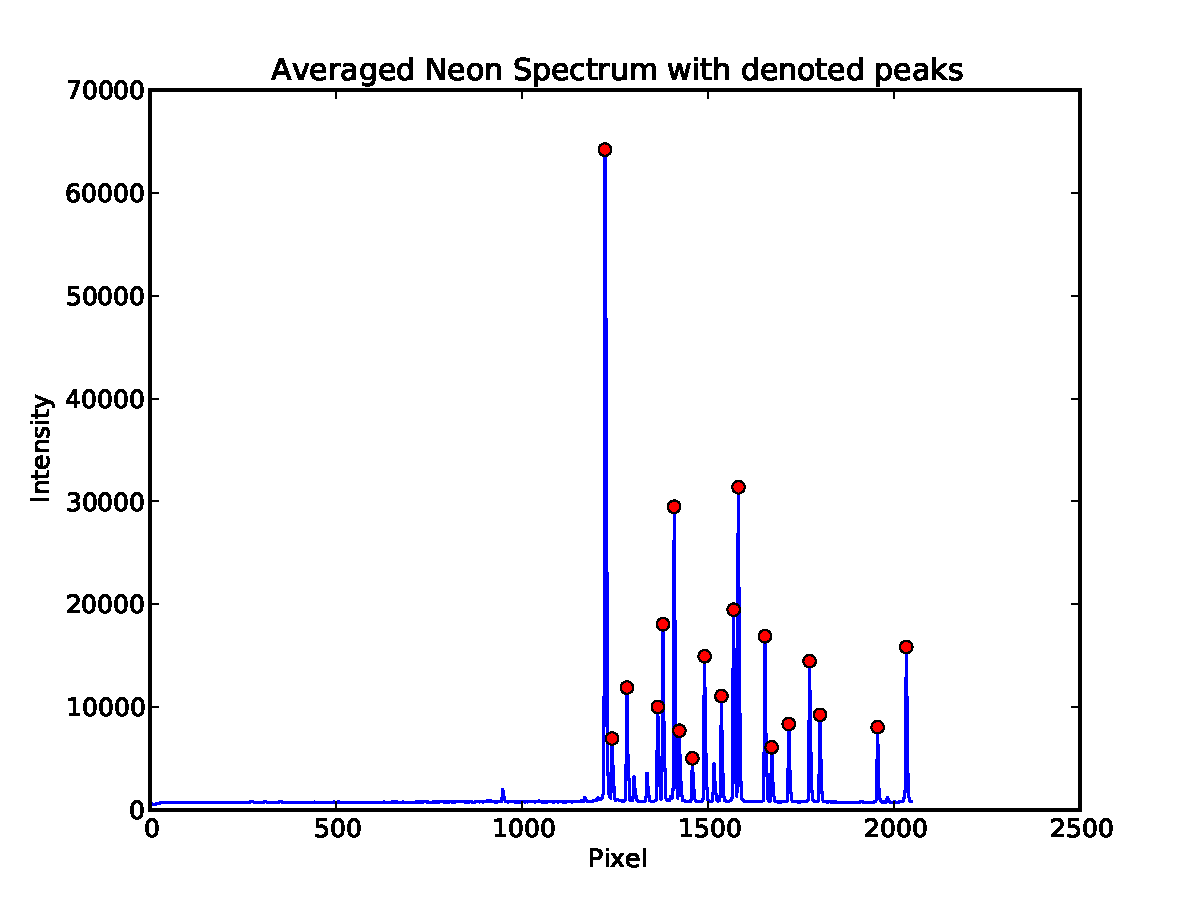
\includegraphics[angle=0,height=6cm,width=12cm]{graphs/Neon_peak_1000.pdf}
\caption{Averaged spectrum of 1000 Neon sample, from Table \ref{table:ccd}, taken using CCD with the peaks denoted by the red dot.}
\label{fig:Neon_averaged}
\end{figure}
%~~~~~~~~~~~~~~~~~~~~~~~~~~~~~~~~~~~~~~~~~~~~~~~~~~~~~~~~~~~~~~~~~~~~~~~~~~~~~~~~~~~~~~~~
%~~~~~~~~~~~~~~~~~~~~~~~~~~~~~~~~~~~~~~~~~~~~~~~~~~~~~~~~~~~~~~~~~~~~~~~~~~~~~~~~~~~~~~~~
\begin{figure}[H]
\centering
$\begin{array}{cc}
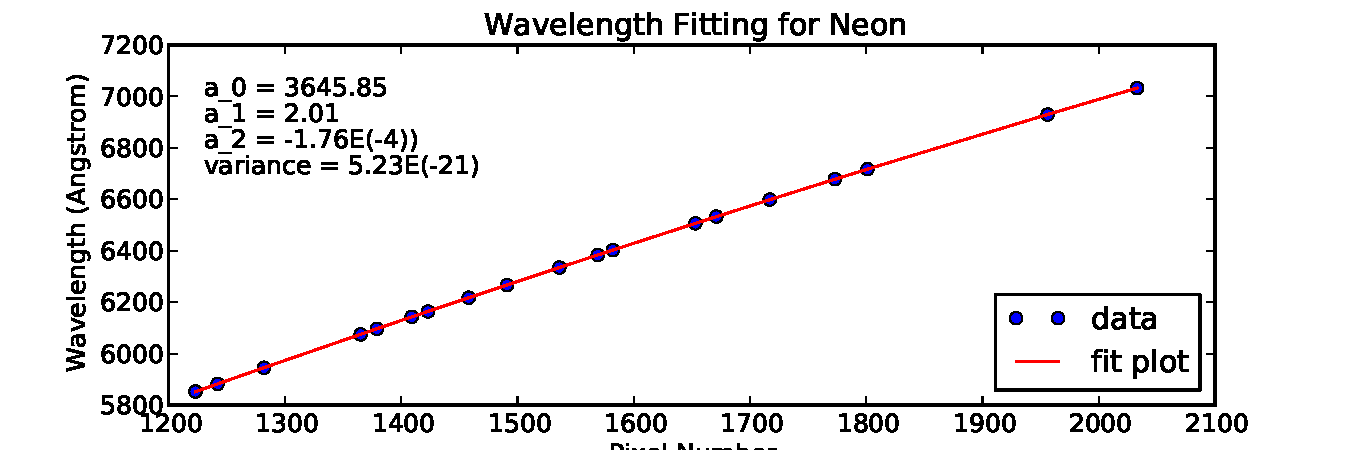
\includegraphics [angle=0,height=3cm,width=13cm]{graphs/CCDNeonFit1.pdf} \\
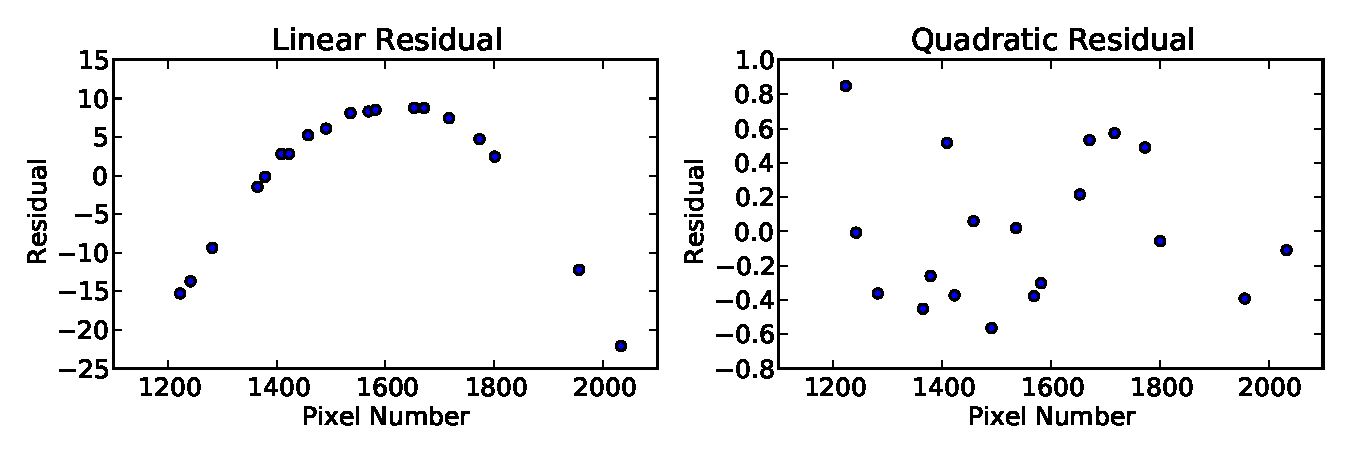
\includegraphics[angle=0,height=3cm,width=12cm]{graphs/CCDNeonFit2.pdf} \\
\end{array}$
\caption{Pixel vs. Wavelength plot on the top, with Linear and Quadratic residual for CCD Spectroscope using the Neon data. $a_0$, $a_1$ and $a_2$ values are the constant for the pixel to wavelength equation.}
\label{fig:Neon_CCD}
\end{figure}
%~~~~~~~~~~~~~~~~~~~~~~~~~~~~~~~~~~~~~~~~~~~~~~~~~~~~~~~~~~~~~~~~~~~~~~~~~~~~~~~~~~~~~~~~
Figure \ref{fig:Neon_averaged} show the marked emmision line of Neon from CCD. Figure \ref{fig:Neon_CCD} plots pixel vs. wavelength with a good fit using python as explained in Section \ref{sec:reduction}. It clearly show that the two values have a very strong correlation. For the linear residual are only within the range of -20 to 15. However, due to the parabolic pattern in linear residual, quadratic was obtained, which shows the even smaller range (-0.8 to 1.0) and randomness. This gave us the the relationship where $wavelength = 3624.85 + 2.01(pixel) + (-1.76E(-4))((pixel)^2)$. These results also show that Neon was the good choice for getting this relation for it have very defined emmission lines that has very little variation. As it can be seen that the variance value is in the $10^{th}$ power of -21.
%~~~~~~~~~~~~~~~~~~~~~~~~~~~~~~~~~~~~~~~~~~~~~~~~~~~~~~~~~~~~~~~~~~~~~~~~~~~~~~~~~~~~~~~~
\begin{figure}[H]
\centering
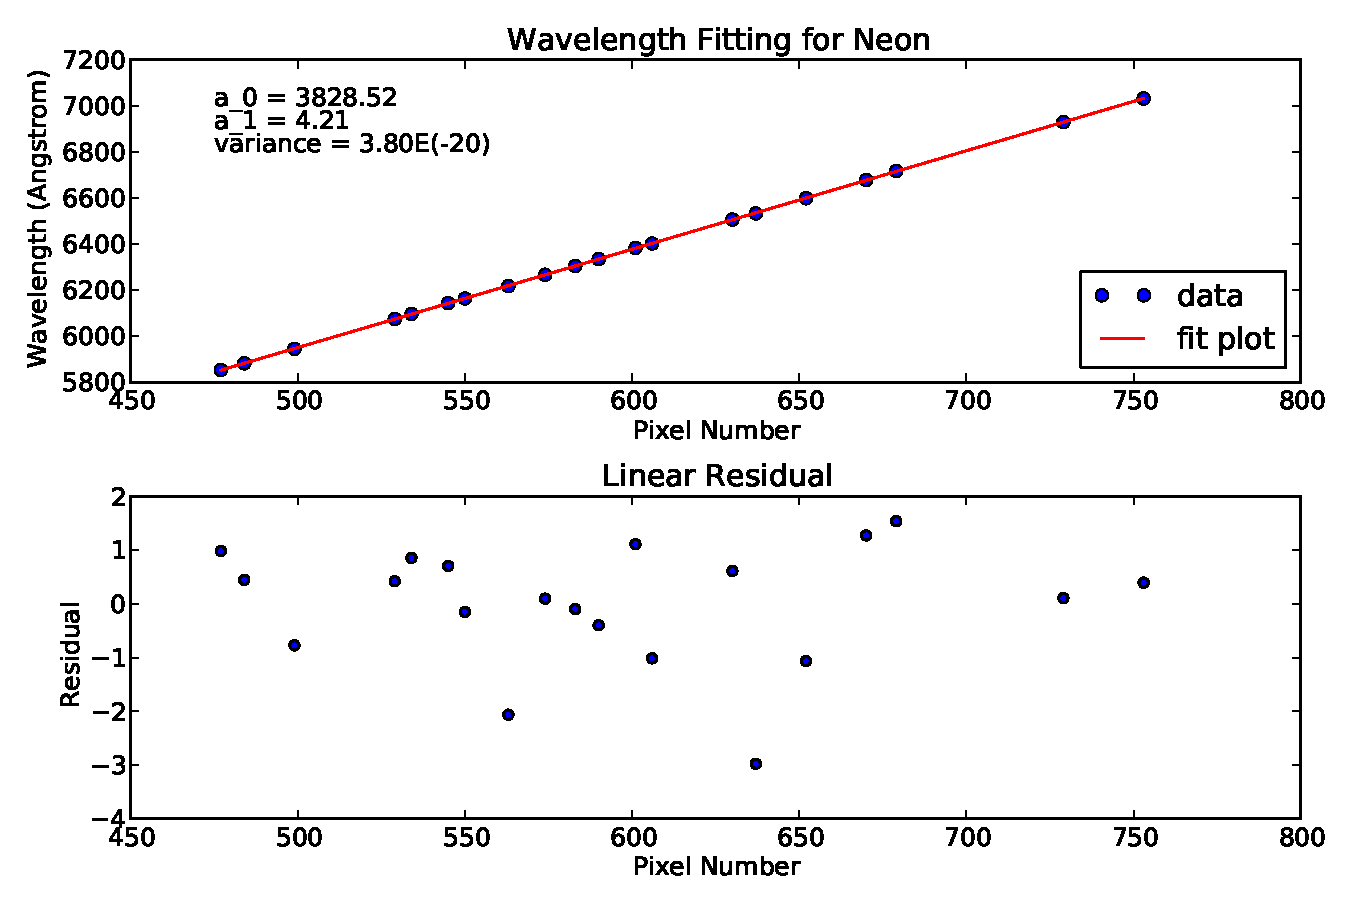
\includegraphics [angle=0,height=7cm,width=13cm]{graphs/Night1NeonFit.pdf} 
\caption{Pixel vs. Wavelength plot with Linear for Telescope Spectroscope using the Neon data  from Table \ref{table:telescope}. $a_0$ and $a_1$ values are the constant for the pixel to wavelength equation.}
\label{fig:Neon_tele}
\end{figure}
%~~~~~~~~~~~~~~~~~~~~~~~~~~~~~~~~~~~~~~~~~~~~~~~~~~~~~~~~~~~~~~~~~~~~~~~~~~~~~~~~~~~~~~~~
Similiary, the wavelength solution for telescope was also obtained, as shown in Figure \ref{fig:Neon_tele}. Here, the linear residual gave good result with the range from -4 to 2 and randomness. Therefore, quadratic fit was not required. This gave us the solution to be $wavelenth = 3828.52 + 4.21(pixel)$ with variance in $10^{th}$ the power of -20.

%##########Gain, Noise and Saturation
\subsection{Gain, Noise and Saturation} 
\label{sec:gns}
%~~~~~~~~~~~~~~~~~~~~~~~~~~~~~~~~~~~~~~~~~~~~~~~~~~~~~~~~~~~~~~~~~~~~~~~~~~~~~~~~~~~~~~~~
\begin{figure}[H]
\centering
$\begin{array}{cc}
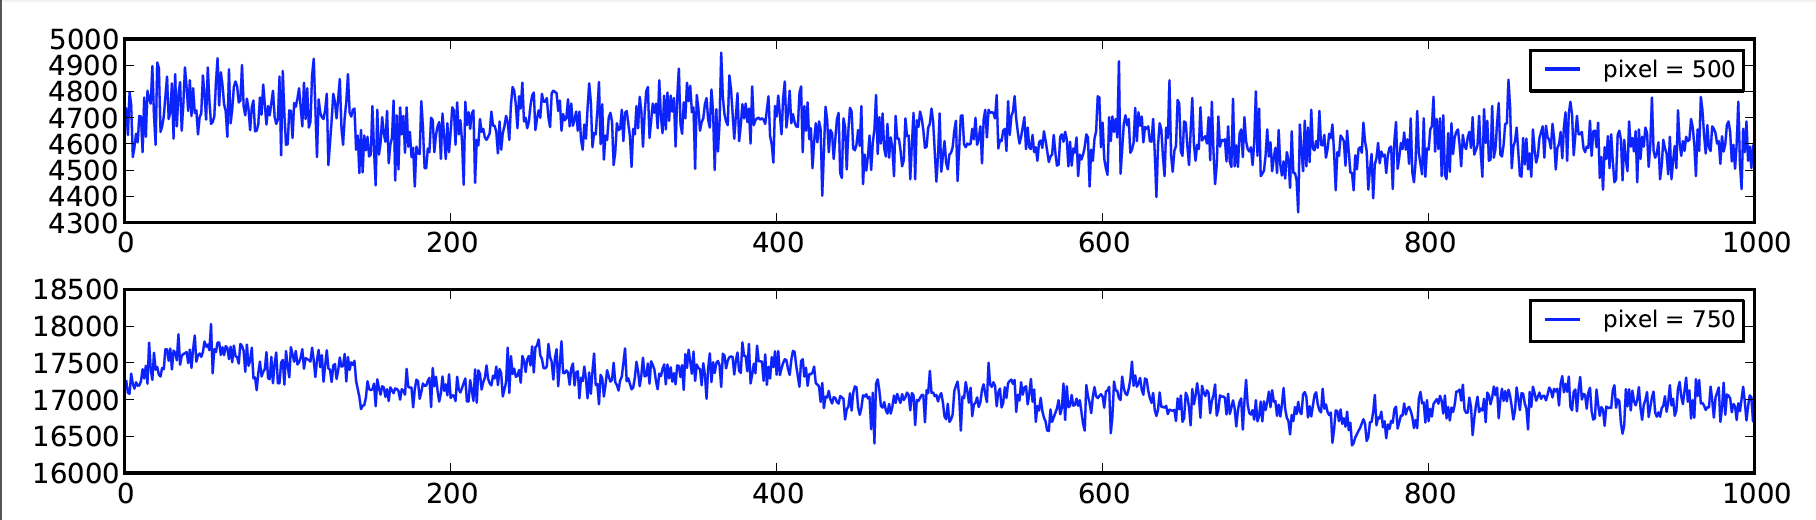
\includegraphics [angle=0,height=4cm,width=7cm]{graphs/ScreenShot1.png} &
\hspace{-0.2cm}
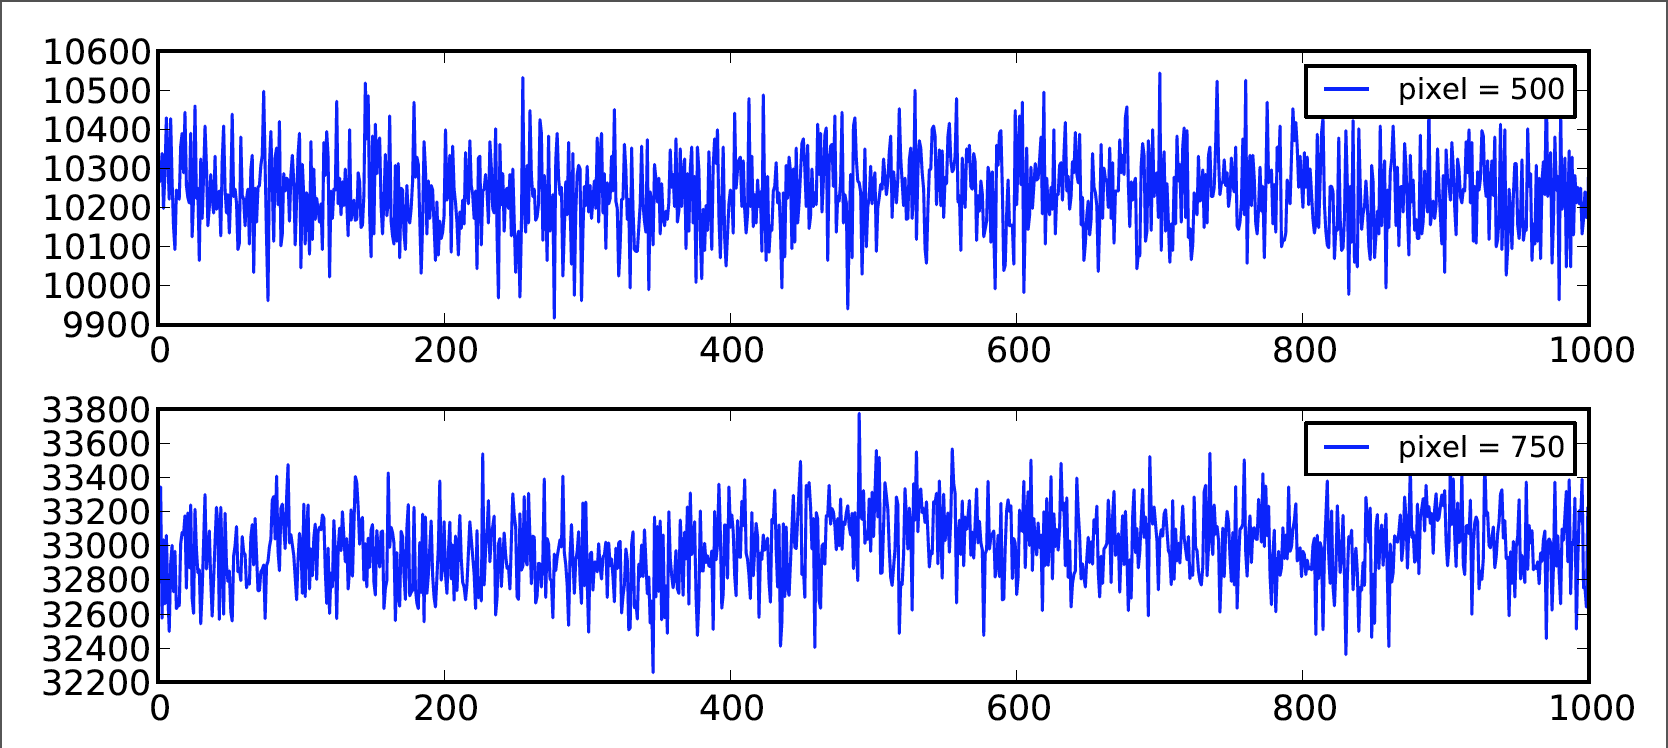
\includegraphics[angle=0,height=4cm,width=7cm]{graphs/ScreenShot2.png} \\
\end{array}$
\caption{Plot of intensity at certain pixel in 1000 sample of Table Lamp data at 100ms, see Table \ref{table:ccd}. Left: from data with many errors. Right: from good data.}
\label{fig:Lamp_CCD}
\end{figure}
%~~~~~~~~~~~~~~~~~~~~~~~~~~~~~~~~~~~~~~~~~~~~~~~~~~~~~~~~~~~~~~~~~~~~~~~~~~~~~~~~~~~~~~~~
For this not being the ideal situation, many errors were introduced. This can be noticed in the Figure \ref{fig:Lamp_CCD}, where each plot shows 1000 lamp samples from CCD at specific pixel. The first plot has lot of instability that was introduced due to someone holding the detector for data collection, as explained in Section \ref{sec:data}. Then the second set of same data was taken, without human error and it is clear that there are still some over all waviness in the plot. 
%~~~~~~~~~~~~~~~~~~~~~~~~~~~~~~~ Figure ~~~~~~~~~~~~~~~~~~~~~~~~~~~~~~~~~~~~~~~~~~~~~~~
\begin{figure}[H]
\centering
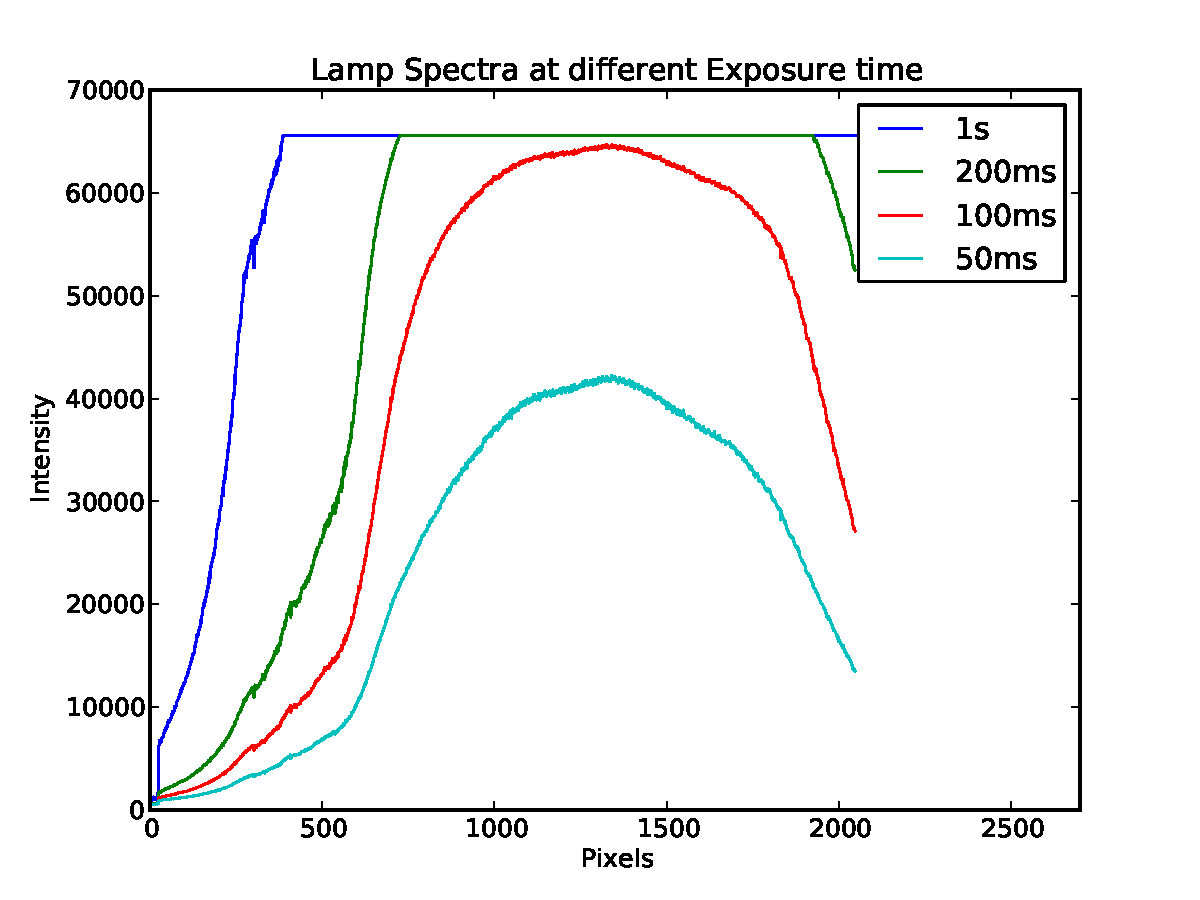
\includegraphics[angle=0,height=6cm,width=12cm]{graphs/Saturation.pdf}
\caption{Averaged spectrum of vaious Lamp data at different exposure time, see Table \ref{table:ccd} for all list of Lamp Data.}
\label{fig:Saturation}
\end{figure}
%~~~~~~~~~~~~~~~~~~~~~~~~~~~~~~~~~~~~~~~~~~~~~~~~~~~~~~~~~~~~~~~~~~~~~~~~~~~~~~~~~~~~~~~~
Longer exposure time allow the detector to collect more photon for that run and therefore the intensity increases for higher time. Figure \ref{fig:Saturation} display that there is a cut off to the amount of intensity the detector can detect called saturation level. Therefore,longer the time, more of the curve will become constant at a value. From this data, we get the saturation level to be exact 65535.
%~~~~~~~~~~~~~~~~~~~~~~~~~~~~~~~~~~~~~~~~~~~~~~~~~~~~~~~~~~~~~~~~~~~~~~~~~~~~~~~~~~~~~~~~
\begin{figure}[H]
\centering
$\begin{array}{cc}
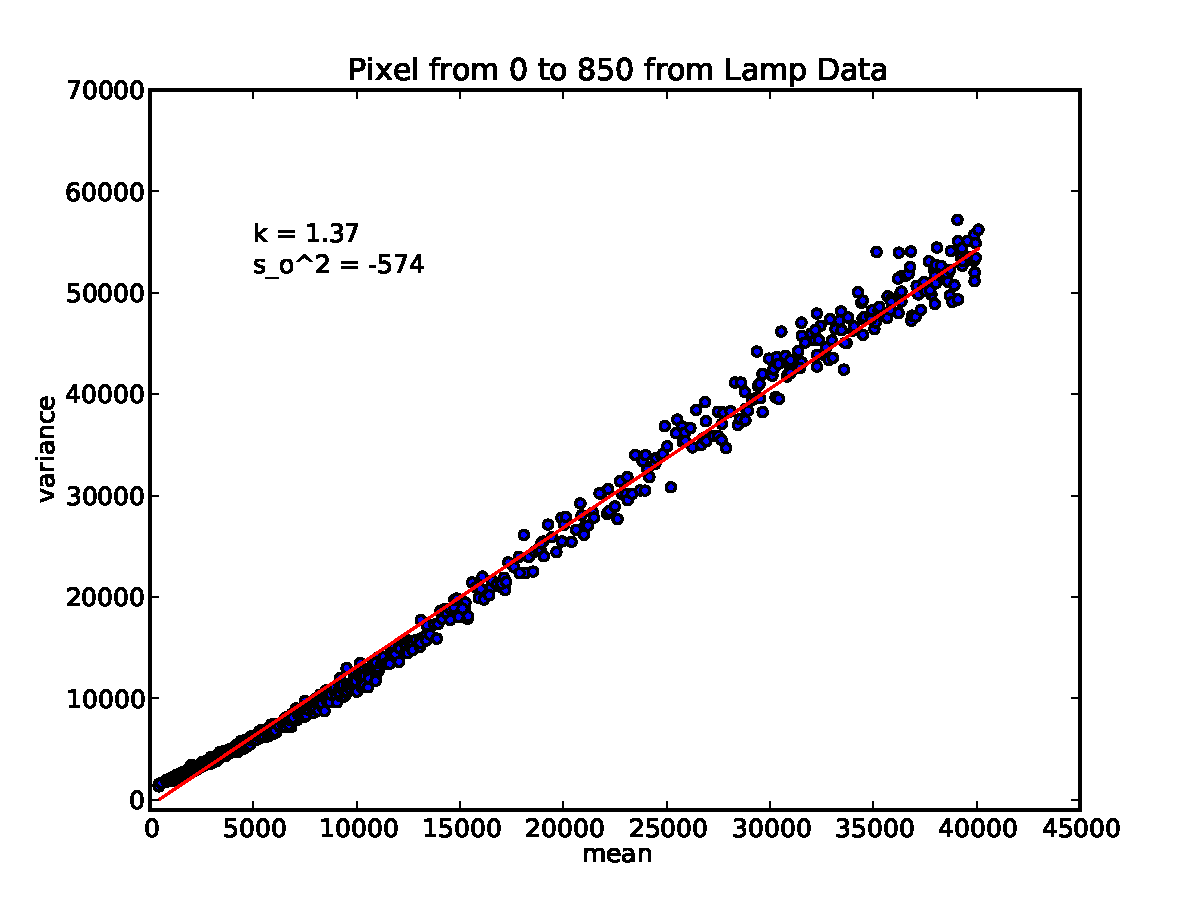
\includegraphics [angle=0,height=7cm,width=7cm]{graphs/Lampfit0-850.pdf} &
\hspace{-0.2cm}
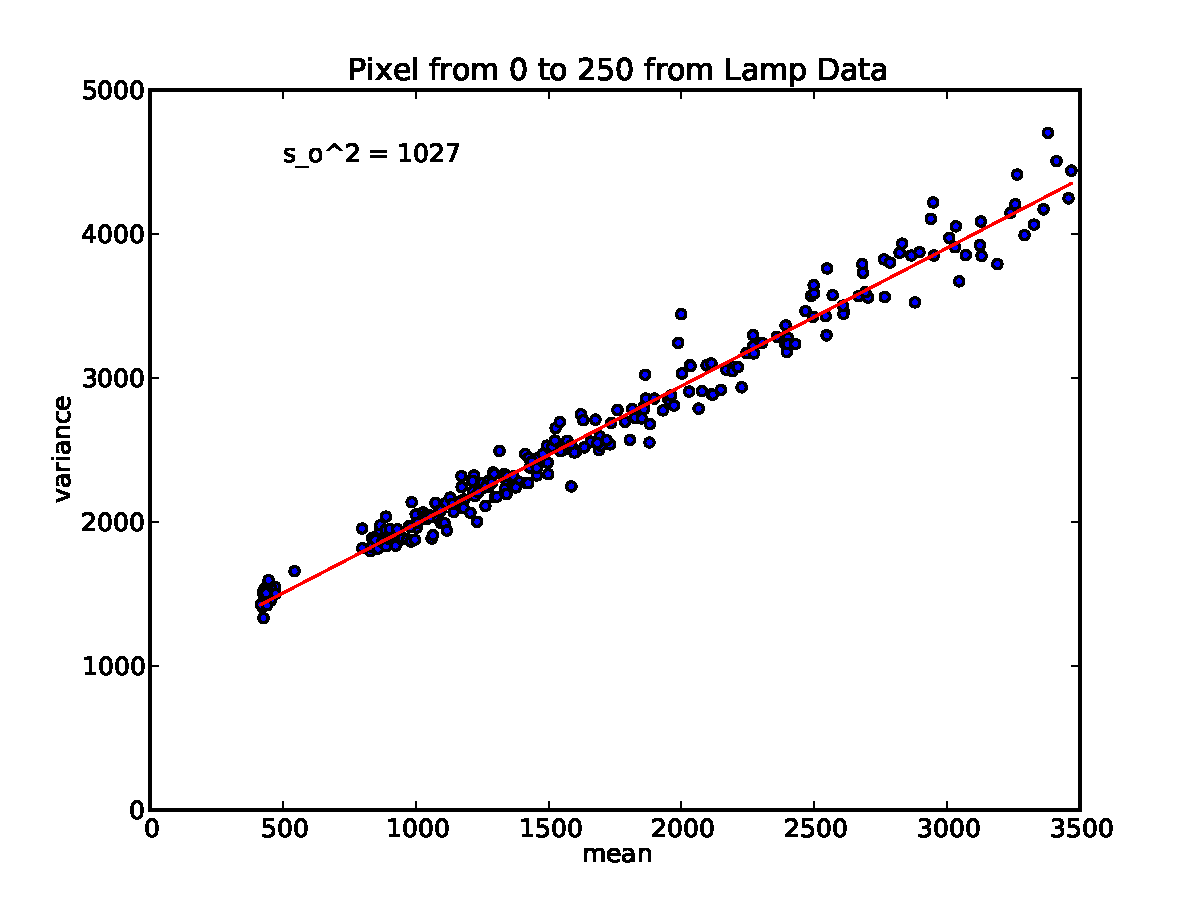
\includegraphics[angle=0,height=7cm,width=7cm]{graphs/LampfitReadNoise.pdf} \\
\end{array}$
\caption{Left: plot of mean vs. variance, using equation \ref{eq:gain}, for pixels 0-850. Right: plot of mean vs. variance for pixels 0-250 used to indentify read noise.}
\label{fig:noise_gain}
\end{figure}
%~~~~~~~~~~~~~~~~~~~~~~~~~~~~~~~~~~~~~~~~~~~~~~~~~~~~~~~~~~~~~~~~~~~~~~~~~~~~~~~~~~~~~~~~
To compensate for the error, gain and read noise was calculated. Keeping satuation level and non-linearlity \cite{instructions} after 40000 in under consideration, average and varianve of pixels from 0-850 was calcualted and plotted using equations \ref{eq:mean}-\ref{eq:gain}, as shown in first plot of Figure \ref{fig:noise_gain}. This gave us the $k$ to be 1.37, which is $\frac{1}{gain}$, as mentioned in Section \ref{sec:noise_ccd}. Therefore, the gain is 0.73. However, the read noise $s^2_0$ is negative because the results dont go to 0 but tangent off to another point. For this process was repeated but for pixels 0-250. This gave us the read noise to be 1027 shown in the scond plot.  


%##########Blackbody Calibration
\subsection{Blackbody Calibration} 
\label{sec:bc}

%~~~~~~~~~~~~~~~~~~~~~~~~~~~~~~~ Figure ~~~~~~~~~~~~~~~~~~~~~~~~~~~~~~~~~~~~~~~~~~~~~~~
\begin{figure}[H]
\centering
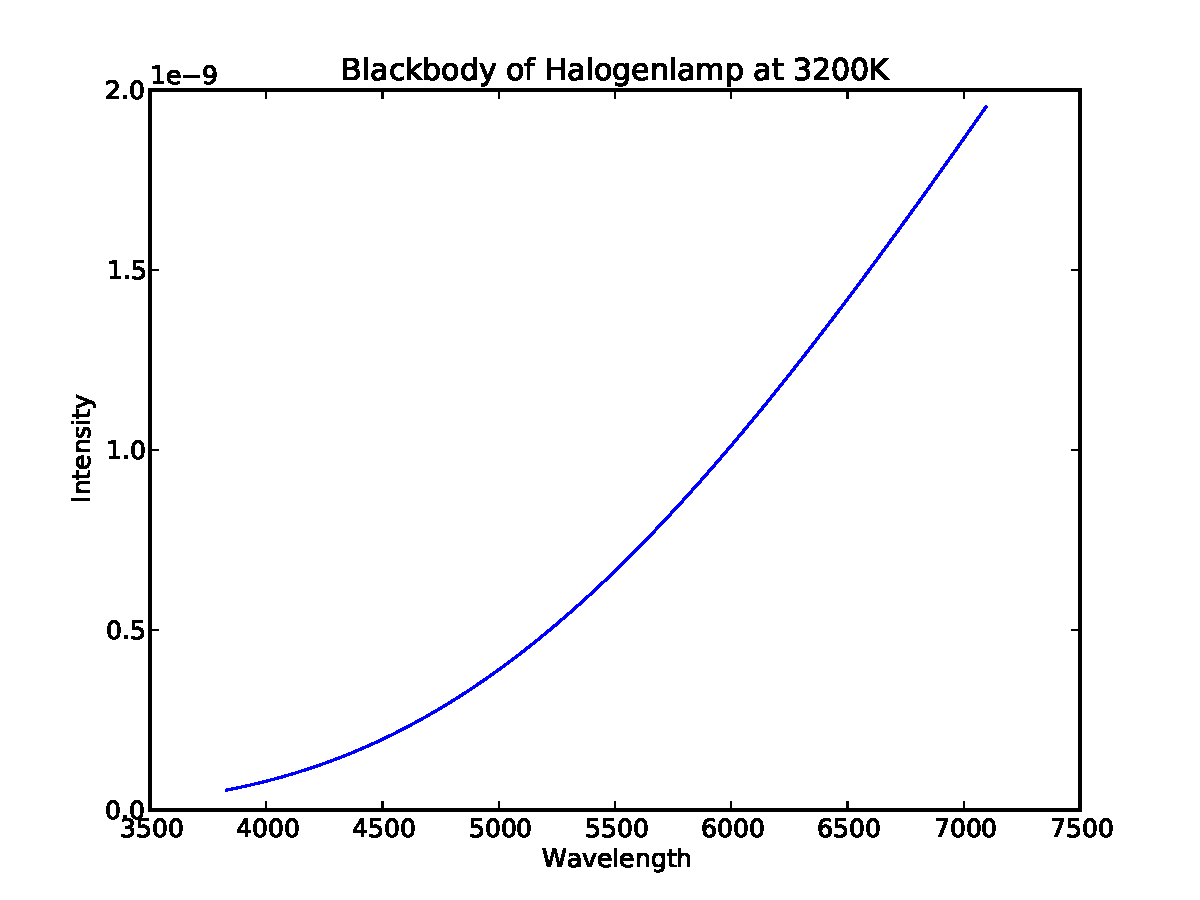
\includegraphics[angle=0,height=6cm,width=8cm]{graphs/Blackbody.pdf}
\caption{Halogen blackbody at temperature 3200K. It was plotted using equation \ref{eq:planck}.}
\label{fig:bb}
\end{figure}
%~~~~~~~~~~~~~~~~~~~~~~~~~~~~~~~~~~~~~~~~~~~~~~~~~~~~~~~~~~~~~~~~~~~~~~~~~~~~~~~~~~~~~~~~
For the telescope data, errors were corrected using diffrent method. Data from halogen lamp was collected, which was suppose to be the perfect blackbody. It was then compared with the actual blackbody of halogen at temperature 3200 K, shown in figure \ref{fig:bb}. Here, it was crutial to keep all the parameters in equation \ref{eq:planck} in SI units, that mean wavelength should be in meters and not in Anstroms. Otherwise, the corrected result was wrong; eventhough it seemed correct. This was then used to correct for the flat field using equation \ref{eq:blackbody} as explained in Section \ref{sec:noise_tele}.
%~~~~~~~~~~~~~~~~~~~~~~~~~~~~~~~ Figure ~~~~~~~~~~~~~~~~~~~~~~~~~~~~~~~~~~~~~~~~~~~~~~~
\begin{figure}[H]
\centering
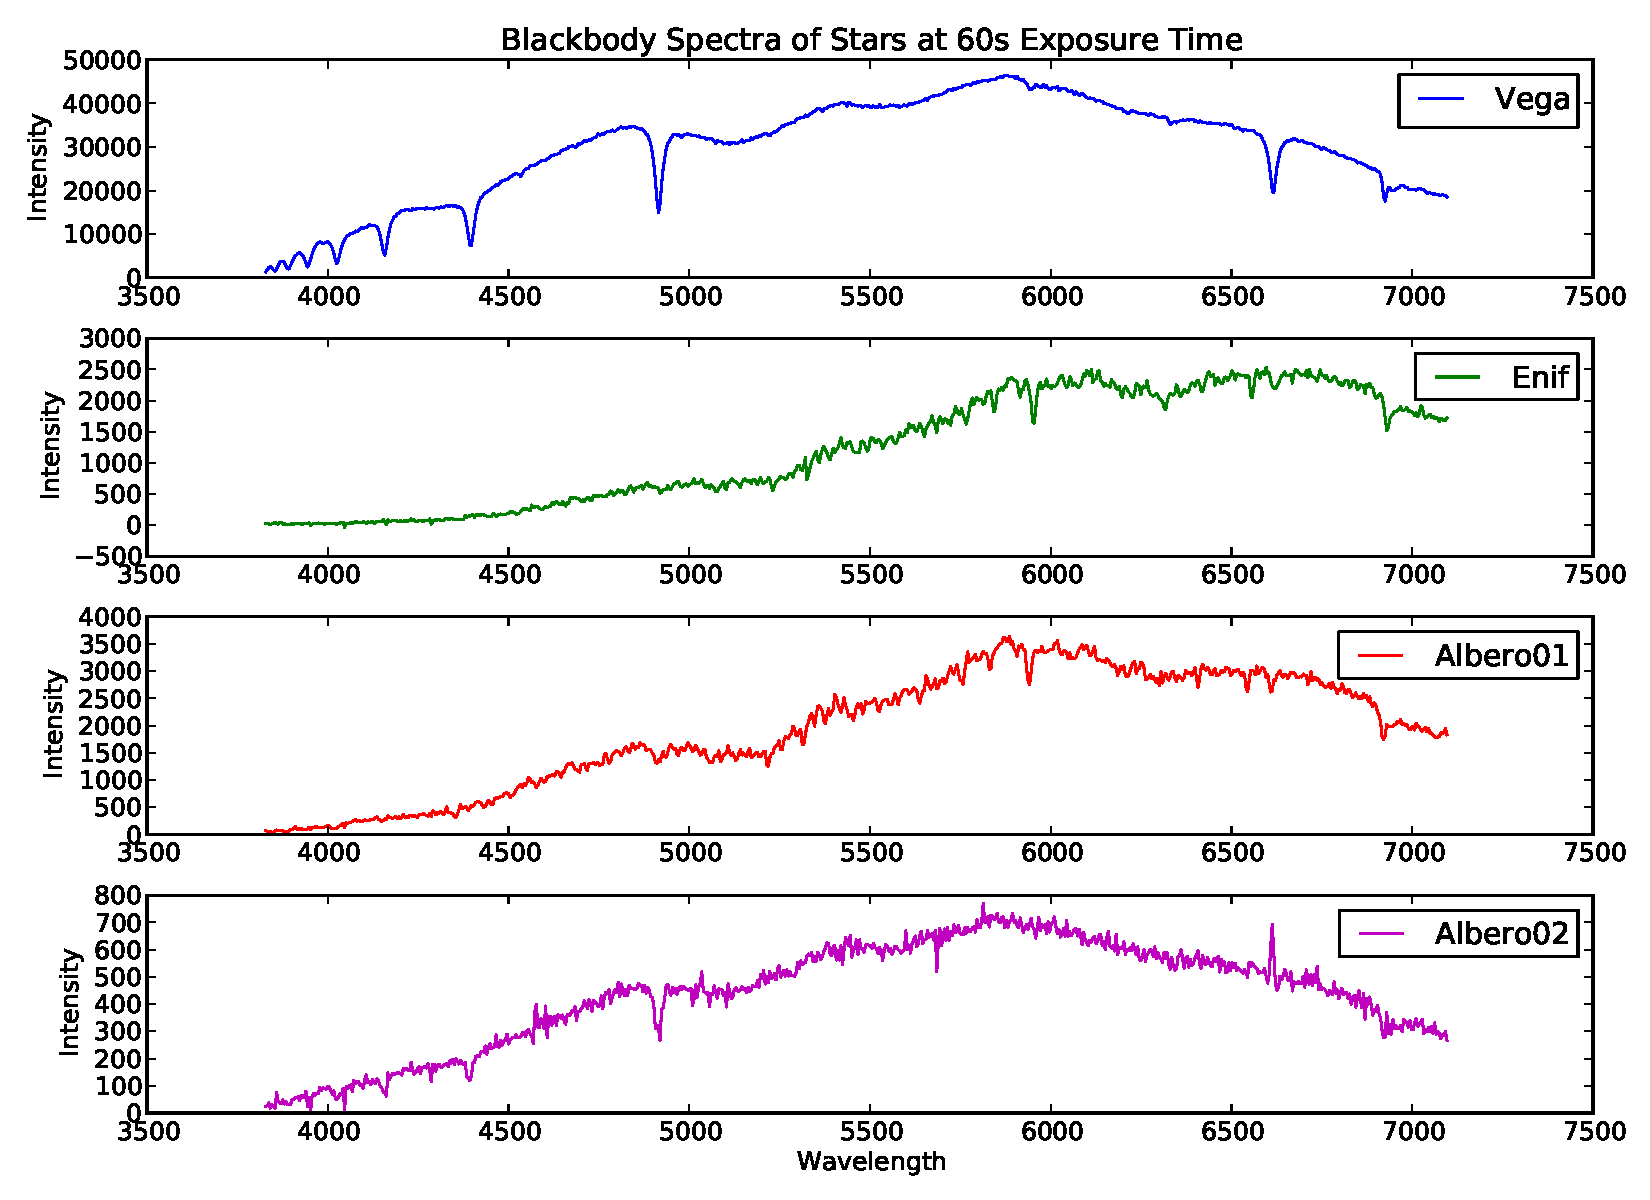
\includegraphics[angle=0,height=8cm,width=12cm]{graphs/Starwithout.pdf}
\caption{Spectrum of Vega, Enif and two Albero before calibration.}
\label{fig:starwithout}
\end{figure}
%~~~~~~~~~~~~~~~~~~~~~~~~~~~~~~~~~~~~~~~~~~~~~~~~~~~~~~~~~~~~~~~~~~~~~~~~~~~~~~~~~~~~~~~~
%~~~~~~~~~~~~~~~~~~~~~~~~~~~~~~~ Figure ~~~~~~~~~~~~~~~~~~~~~~~~~~~~~~~~~~~~~~~~~~~~~~~
\begin{figure}[H]
\centering
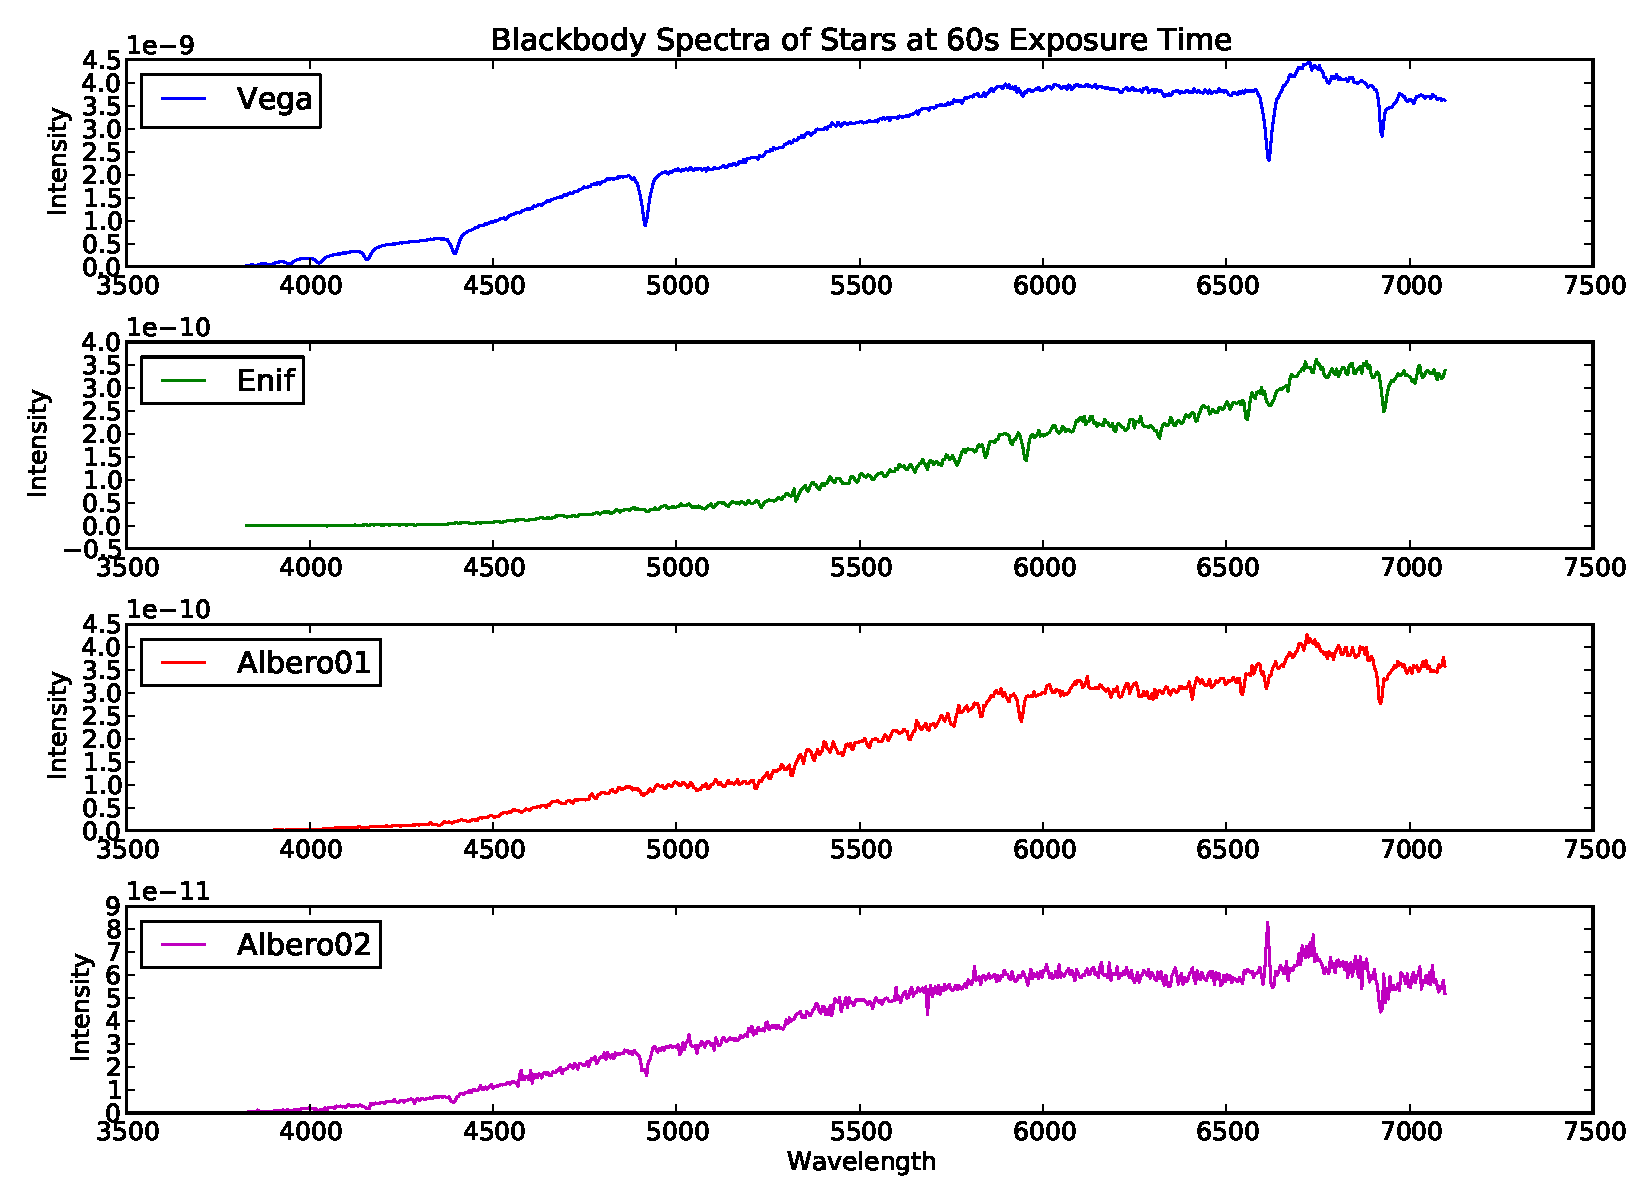
\includegraphics[angle=0,height=8cm,width=12cm]{graphs/Star.pdf}
\caption{Spectrum of Vega, Enif and two Albero after calibration.}
\label{fig:star}
\end{figure}
%~~~~~~~~~~~~~~~~~~~~~~~~~~~~~~~~~~~~~~~~~~~~~~~~~~~~~~~~~~~~~~~~~~~~~~~~~~~~~~~~~~~~~~~~
This method corrected the raw data from Figure \ref{fig:starwithout} to calibrated data in Figure \ref{fig:star}. In Figure \ref{fig:star}, we see that the peak of these spectra are shifted in the direction of the halogen blackbody peak from Figure \ref{fig:bb}. Using the non-calibrated one will give some what same absorbtion lines however it will give very differnet result for the surface temperature of the Star using equation \ref{eq:wein}.
%~~~~~~~~~~~~~~~~~~~~~~~~~~~~~~~~~~~~~~~~~~~~~~~~~~~~~~~~~~~~~~~~~~~~~~~~~~~~~~~~~~~~~~~~
\begin{table}[H]
\centering % used for centering table
\caption{Approximate Surface Temperature of the Stars in Kelvin.}
\tabcolsep 2.pt %\small
\footnotesize

\begin{tabular}{ccccc}% centred columns (8 columns)
\hline
\hline
Vega & Enif & Albero01 & Albero02 & Sun \\
\hline
4400   &    4300   &    4300 & 4300&5400\\
\hline
\hline

\end{tabular}
\label{table:blackbody} % is used to refer this table in the text
\end{table}
%~~~~~~~~~~~~~~~~~~~~~~~~~~~~~~~~~~~~~~~~~~~~~~~~~~~~~~~~~~~~~~~~~~~~~~~~~~~~~~~~~~~~~~~~
%####################### Discussion 
\section{Discussion}
\label{sec:discuss}

%####################### CCD
\subsection{CCD} 
\label{sec:ccd}
%~~~~~~~~~~~~~~~~~~~~~~~~~~~~~~~ Figure ~~~~~~~~~~~~~~~~~~~~~~~~~~~~~~~~~~~~~~~~~~~~~~~
\begin{figure}[H]
\centering
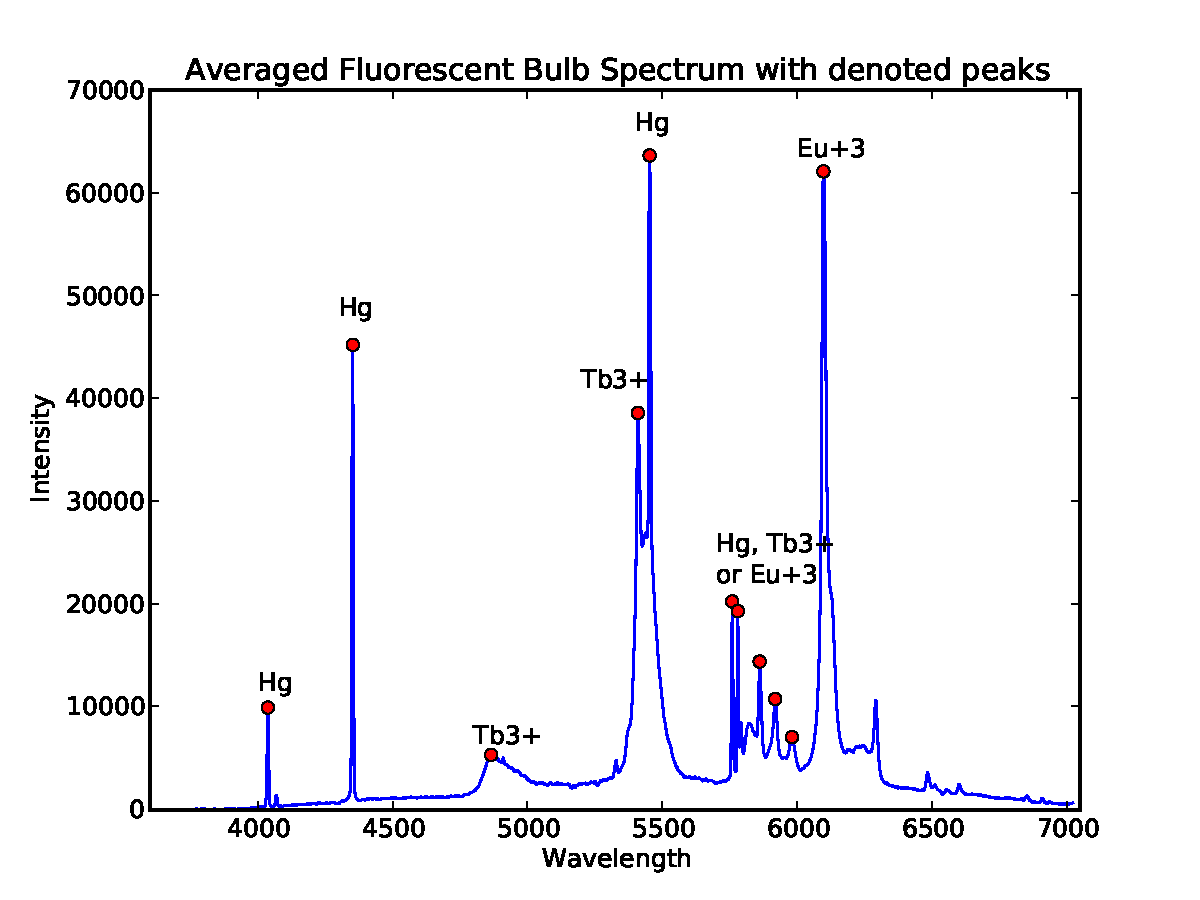
\includegraphics[angle=0,height=5cm,width=10cm]{graphs/FluoLampPeak.pdf}
\caption{Spectrum of Flourescent Bulb with indicated emmision lines.}
\label{fig:bulb}
\end{figure}
%~~~~~~~~~~~~~~~~~~~~~~~~~~~~~~~~~~~~~~~~~~~~~~~~~~~~~~~~~~~~~~~~~~~~~~~~~~~~~~~~~~~~~~~~
Figure \ref{fig:bulb}, shows the plot of the Flourscent Bulb and the detected elements. First thing to notice is that Flourscent Bulb has emission lines, this mean that the photons were coming from the gas around the source. These emission line correspond to specific element as denoted in the Figure \ref{fig:bulb}, which was detected using an additional source to get theoretical values \cite{theo}. Mostly, there is Mg (Mercury) detected, which compliment the fact that these bulbs are made up of mercury-vapour. 
%~~~~~~~~~~~~~~~~~~~~~~~~~~~~~~~ Figure ~~~~~~~~~~~~~~~~~~~~~~~~~~~~~~~~~~~~~~~~~~~~~~~
\begin{figure}[H]
\centering
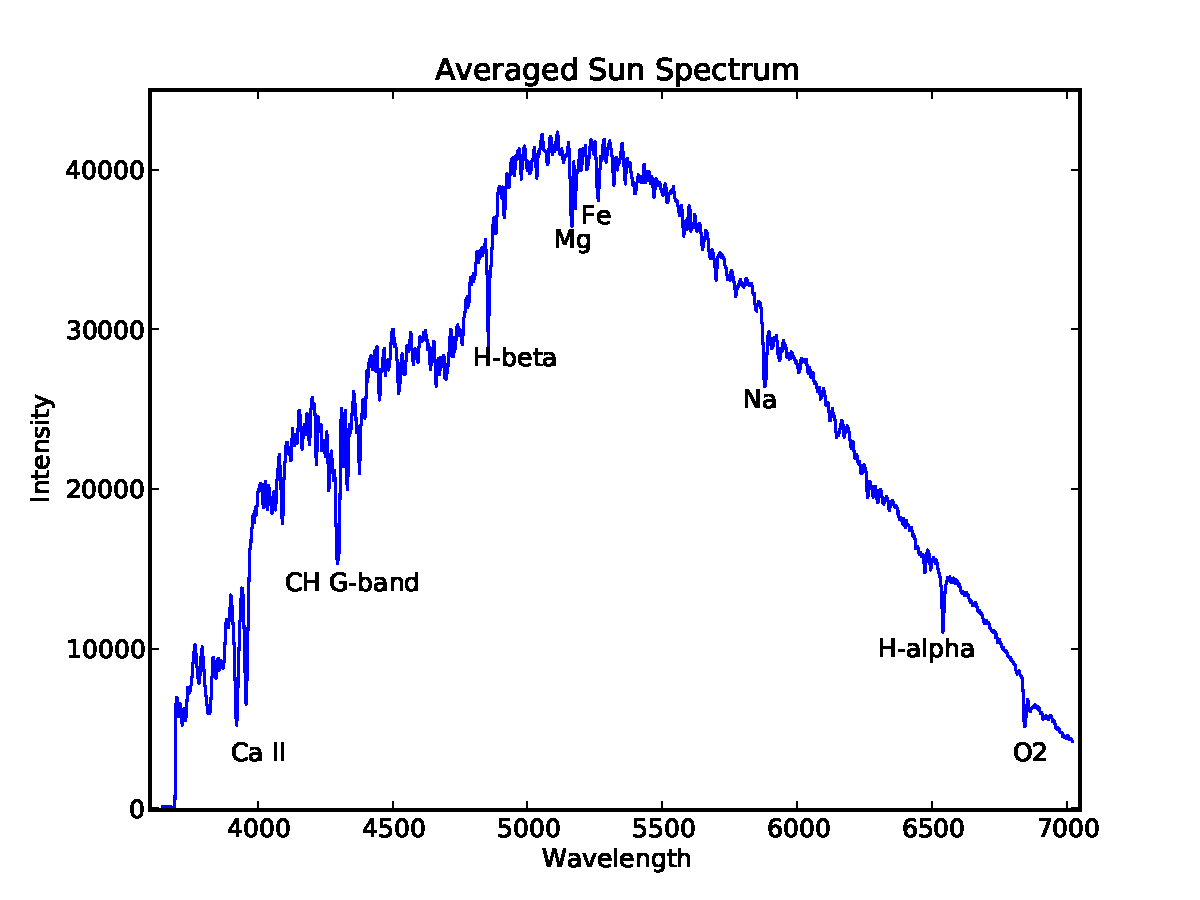
\includegraphics[angle=0,height=5cm,width=10cm]{graphs/Sun.pdf}
\caption{Spectrum of Sun with indicated absorbtion lines.}
\label{fig:sun}
\end{figure}
%~~~~~~~~~~~~~~~~~~~~~~~~~~~~~~~~~~~~~~~~~~~~~~~~~~~~~~~~~~~~~~~~~~~~~~~~~~~~~~~~~~~~~~~~
In Figure \ref{fig:sun}, the averaged spectrum of Sun at 100ms is shown. Here there are absorbtion line instead of emission line. This means photons are not coming directly from the source but passing though a cooler gas, which happens to be the surface of the star. In Sun, the absorbtion line correspond to Fe, Na, Ca, Mg, H-alpha, H-beta and O$_2$.
%####################### Telescope
\subsection{Telescope} 
\label{sec:telescope}

%~~~~~~~~~~~~~~~~~~~~~~~~~~~~~~~ Figure ~~~~~~~~~~~~~~~~~~~~~~~~~~~~~~~~~~~~~~~~~~~~~~~
\begin{figure}[H]
\centering
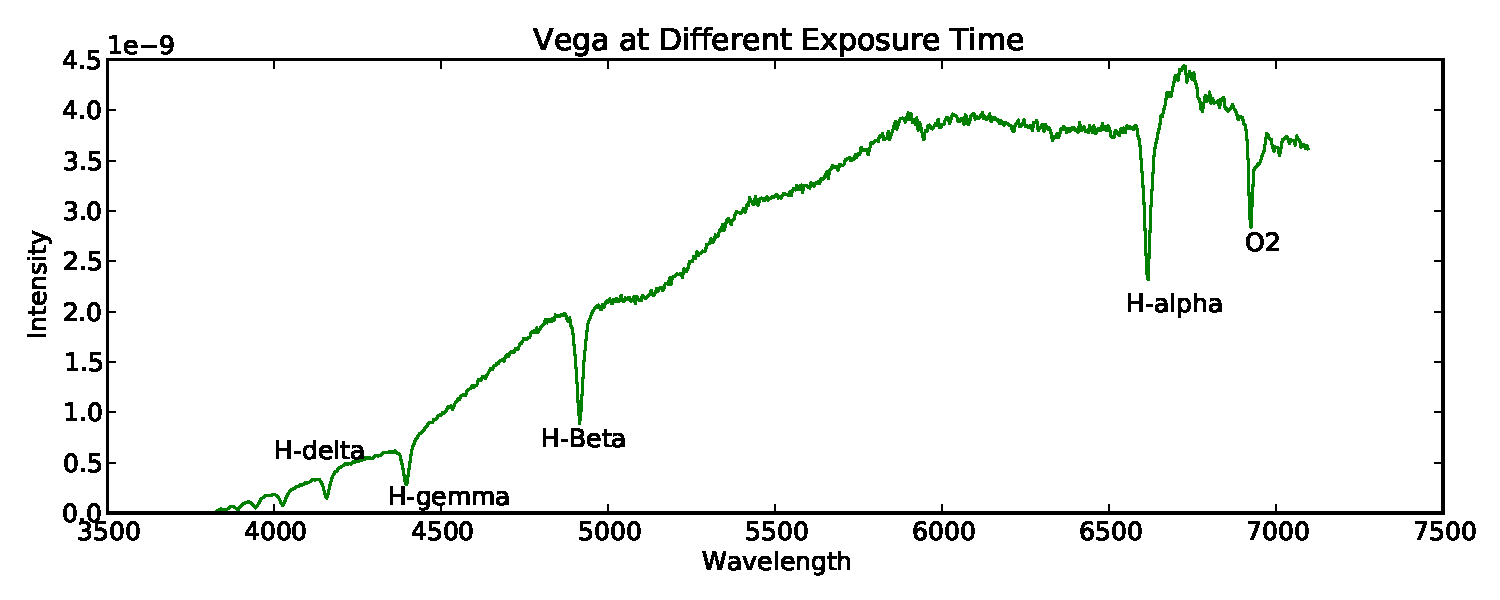
\includegraphics[angle=0,height=5cm,width=12cm]{graphs/Vegaline.pdf}
\caption{Spectrum of Vega with indicated absorbtion lines in Hydrogen Balmer series.}
\label{fig:vega}
\end{figure}
%~~~~~~~~~~~~~~~~~~~~~~~~~~~~~~~~~~~~~~~~~~~~~~~~~~~~~~~~~~~~~~~~~~~~~~~~~~~~~~~~~~~~~~~~
For Vega from Telescope, Figure \ref{fig:vega} also show absorbtion lines. Here, the detected lines are Hydrogen Balmer series that was also compared to the theoretical results \cite{theo}. We see these line in other stars as well. For example, from Figure \ref{fig:vega} and Figure \ref{fig:star}, there is presence of H-beta in Vega and Albero02 because they are hotter star. Also, there is O$_2$ line in all four stars. We can see that this line is has about the same amount of drop in all the star. Therefore, this can be concluded that this from the atmosphere. This also show that O$_2$ could also be from the atmosphere. 
%~~~~~~~~~~~~~~~~~~~~~~~~~~~~~~~ Figure ~~~~~~~~~~~~~~~~~~~~~~~~~~~~~~~~~~~~~~~~~~~~~~~
\begin{figure}[H]
\centering
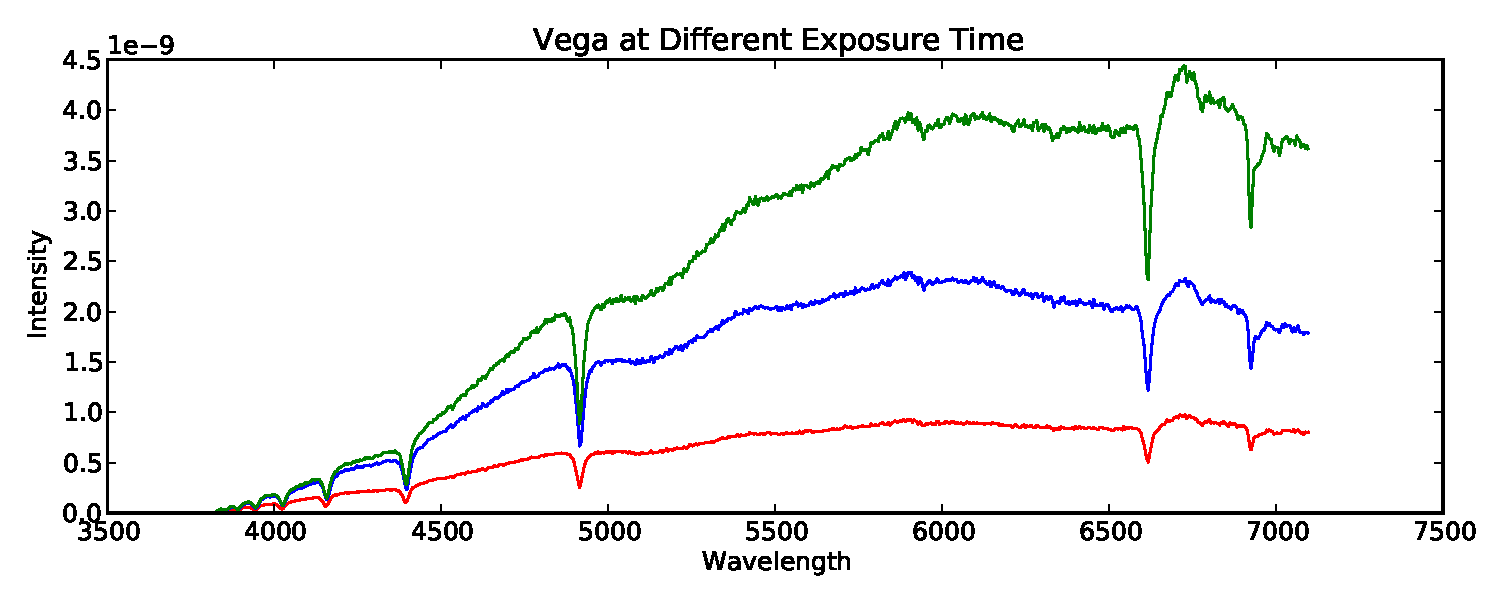
\includegraphics[angle=0,height=5cm,width=12cm]{graphs/Vega.pdf}
\caption{Spectrum of Vega at three different exposure time: 15s, 30s, and 60s}
\label{fig:vegaall}
\end{figure}
%~~~~~~~~~~~~~~~~~~~~~~~~~~~~~~~~~~~~~~~~~~~~~~~~~~~~~~~~~~~~~~~~~~~~~~~~~~~~~~~~~~~~~~~~
Figure \ref{fig:vegaall} show that like USB2000, telescope also collect more photon for longer integration time. One thing to notice is that for longer exposure The feature are becoming more prominant. Therefore higher time will give better result. But surface temperature gave difficult result.From Table \ref{table:blackbody}, for Sun, Enif and even Albero01, the values seems quite close to the theroritical values for they are cooler star. However Vega and Albero02 are very off from their real values. This is because the halogen flatfield calibration doesn't work for UV stars \cite{instructions}. This means there needs to be an another way to correct for all types of Stars.
\bibliographystyle{plain}
\bibliography{references.bib}
\end{document}
